\subsubsection{Sequential switching between Tent and Logistic maps (SWITCH)} \label{sssec:switch}

Results with sequential switching are shown in Figs. \ref{fig:SWITCH_QuantiB} (a) to (f).
The entropy value calculated in floating point is $H_{val}=0.9722$, this value is slightly higher than the one obtained for the LOG map. 
For fixed point arithmetic this value is reached in $B=24$, but it stabilizes from $B=28$.
Regarding the ordering patterns the number of MP decreases to $586$, this value lower than the one obtained for LOG map.
It means the entropy $H_{BP}$ may increase up to $ln(134)/ln(720)\simeq 0.74$.
$BP$ and $BPW$ quantifiers reach their maximum of $H_{BP}=0.6546$ and $H_{BPW}=0.6313$ at $B=16$, but they stabilize from $B=24$.
Complexities are lower than for LOG, $C_{BP}=0.4580$ and $C_{BPW}=0.4578$, these values are reached for $B \geq 15$ but they are stable from $B \geq 23$.
Compared with LOG, statistical properties are better with less amount of bits, for $B \geq 24$ this map reaches optimal characteristics in the sense of random source.

Furthermore, we encountred one initial condition in floating point double precision with an anomalous behaviour.
The quantifiers based on BPW procedure cant detect an anomaly, \ref{fig:SWITCH_QuantiB} (a), (b) and (d) an horizontal blue dashed line is far from the average value but this can not be seen in the rest \ref{fig:SWITCH_QuantiB} (c) and (e).
We detect a falling to a fixed point after a long transitory, the BPW procedure discards the values corresponding with a fixed point and calculates only the transitory.

\begin{figure}
	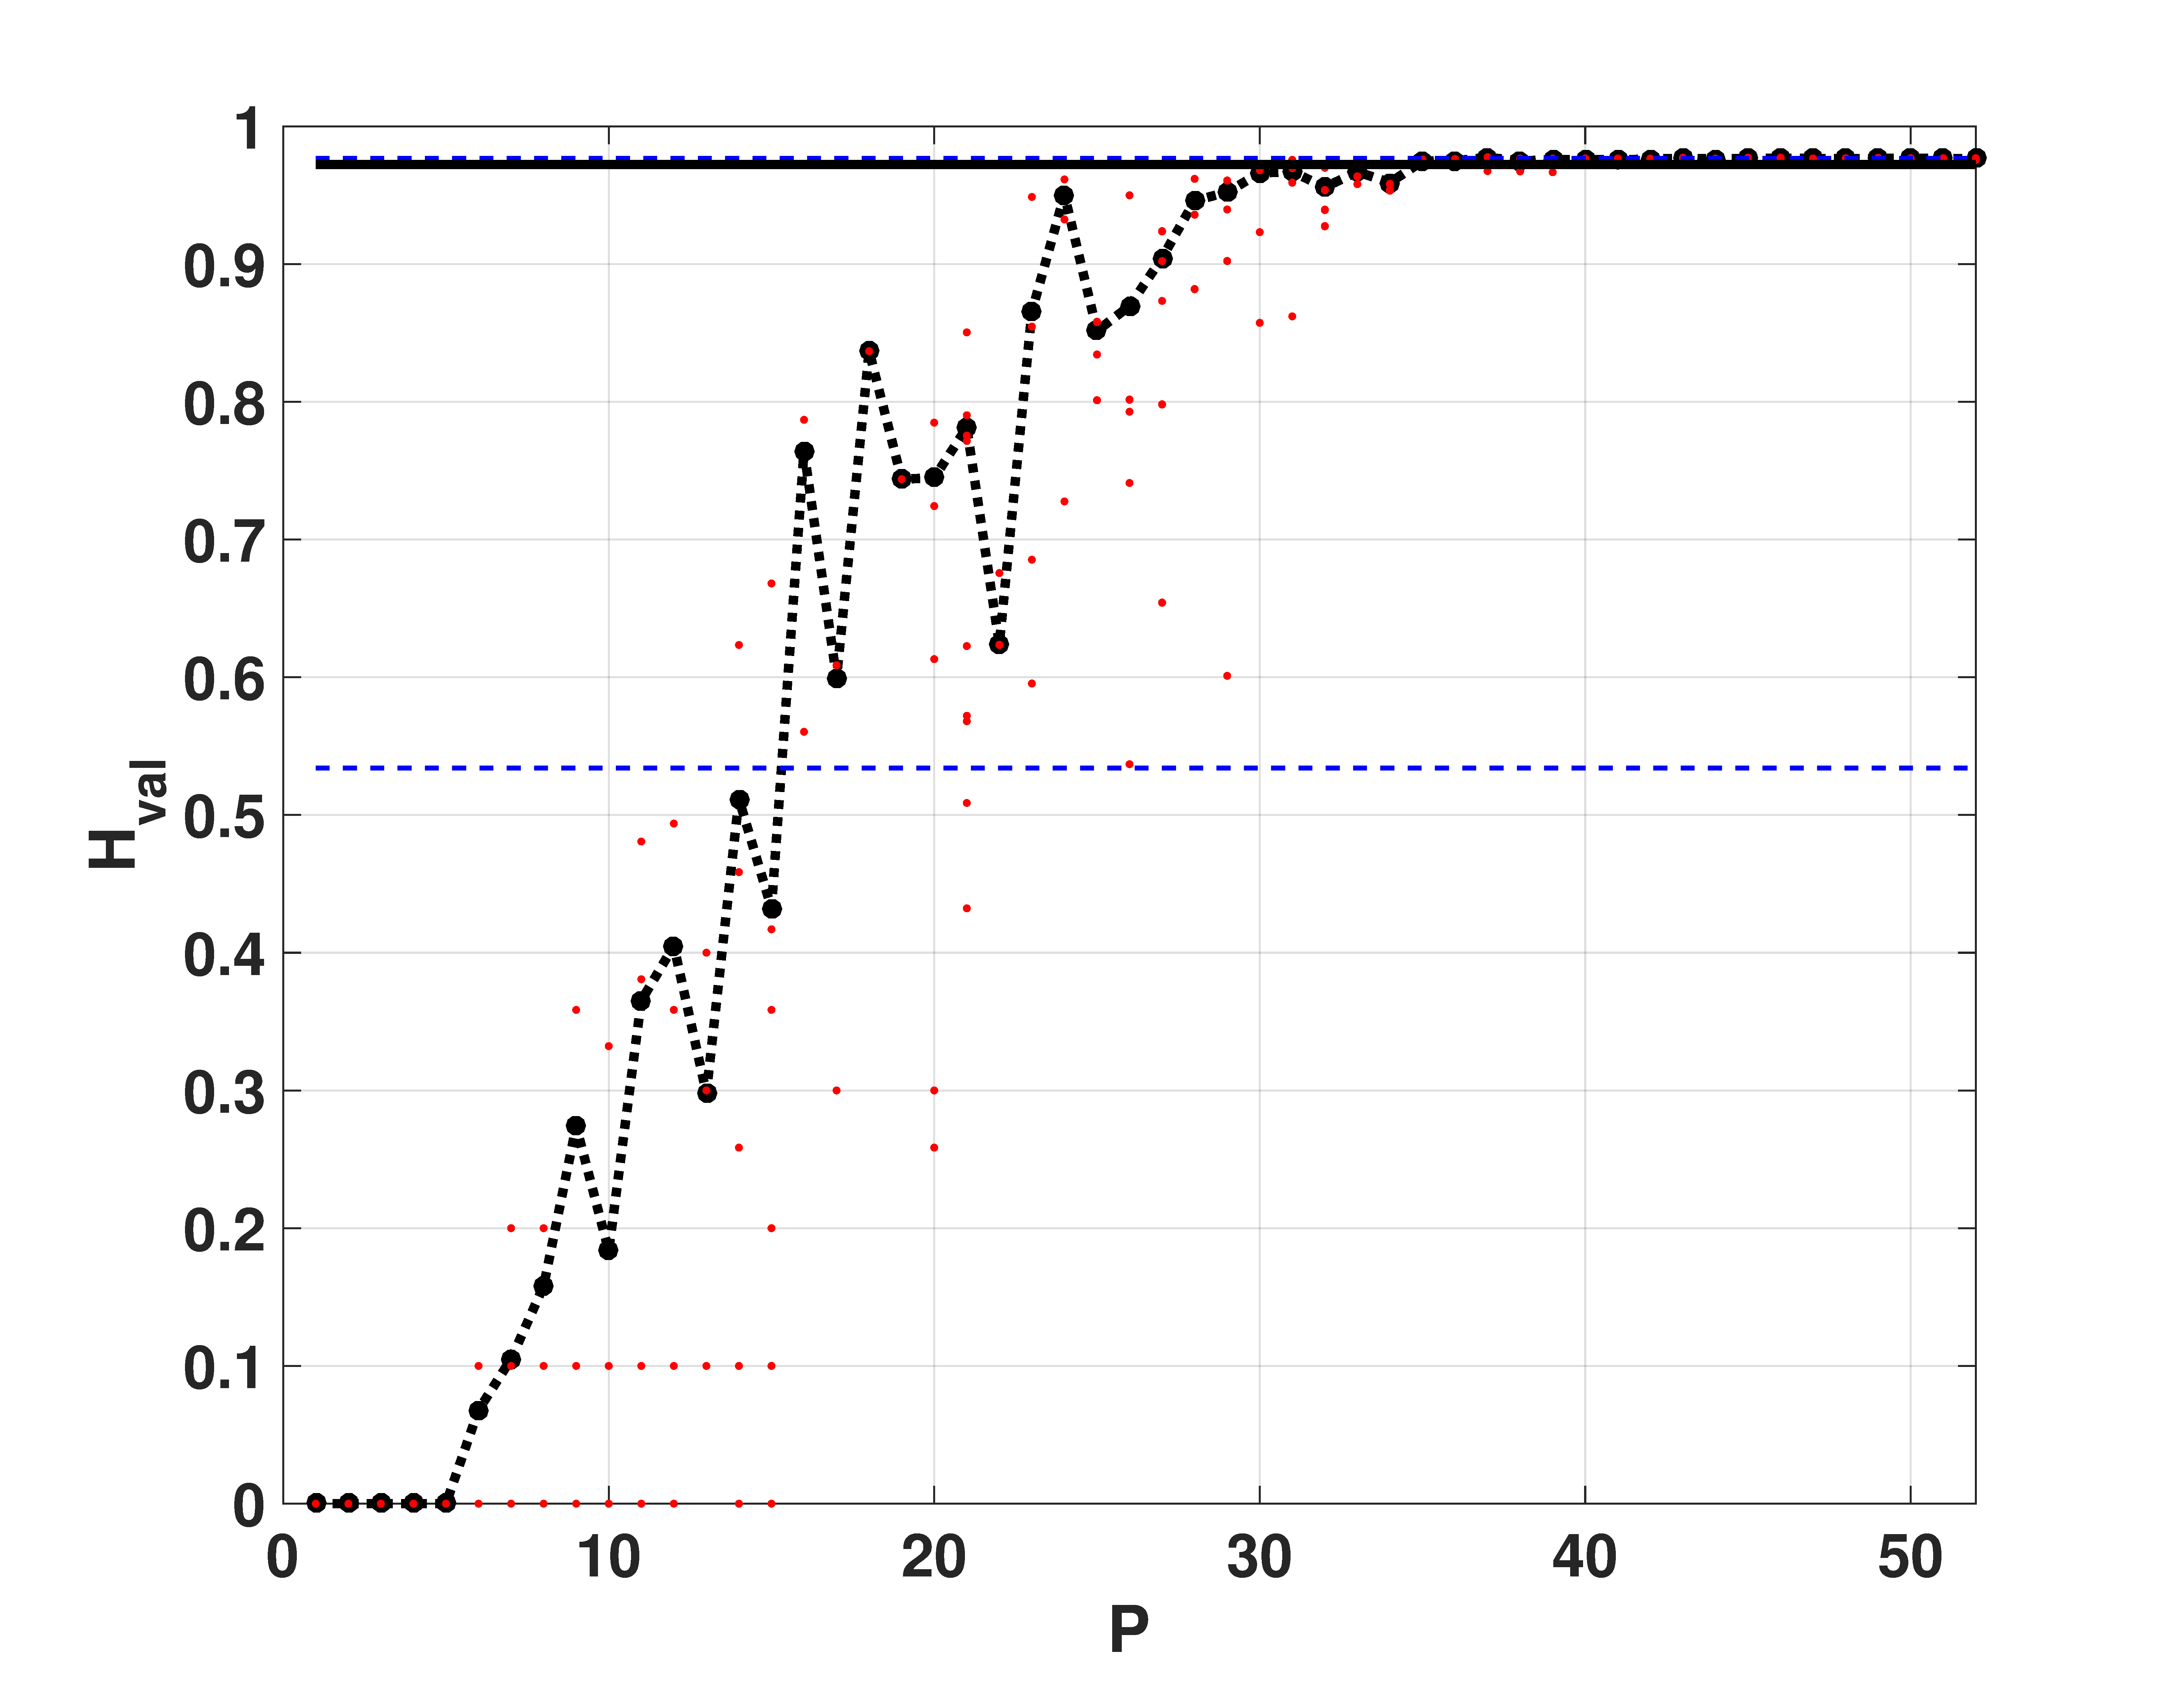
\includegraphics[width=.49\textwidth]{Hval_Switch}
	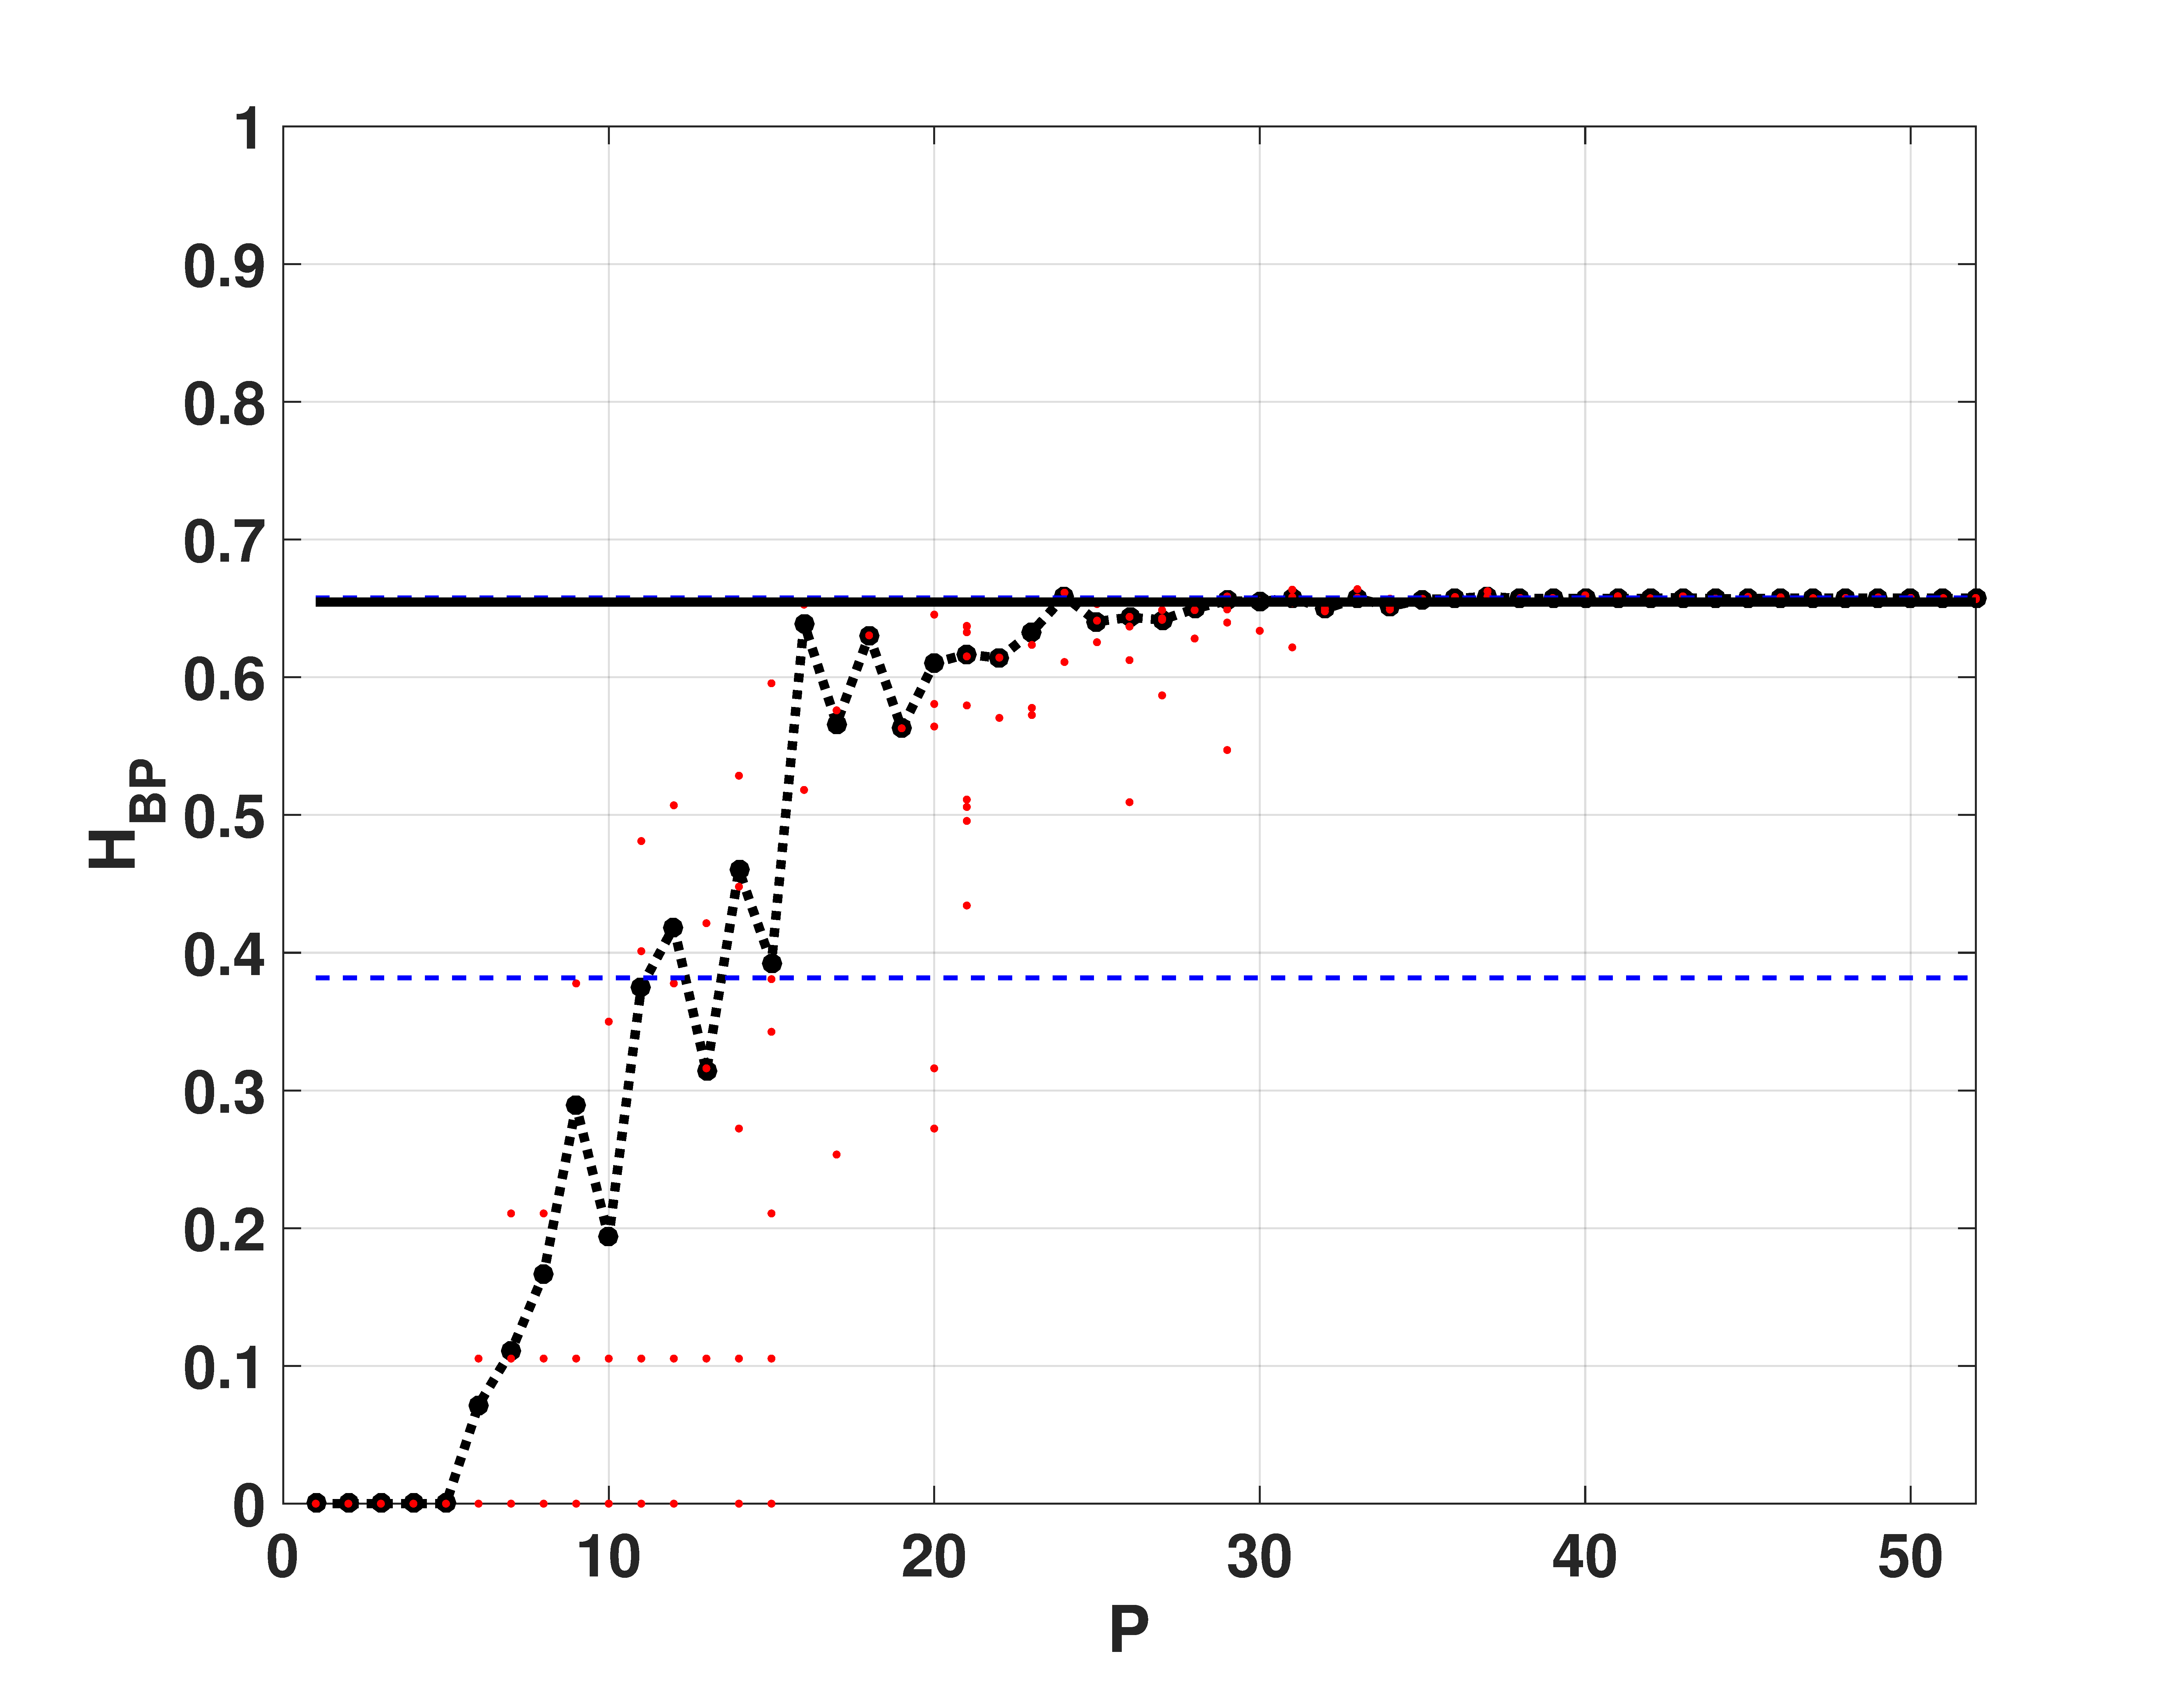
\includegraphics[width=.49\textwidth]{Hbp_Switch}
	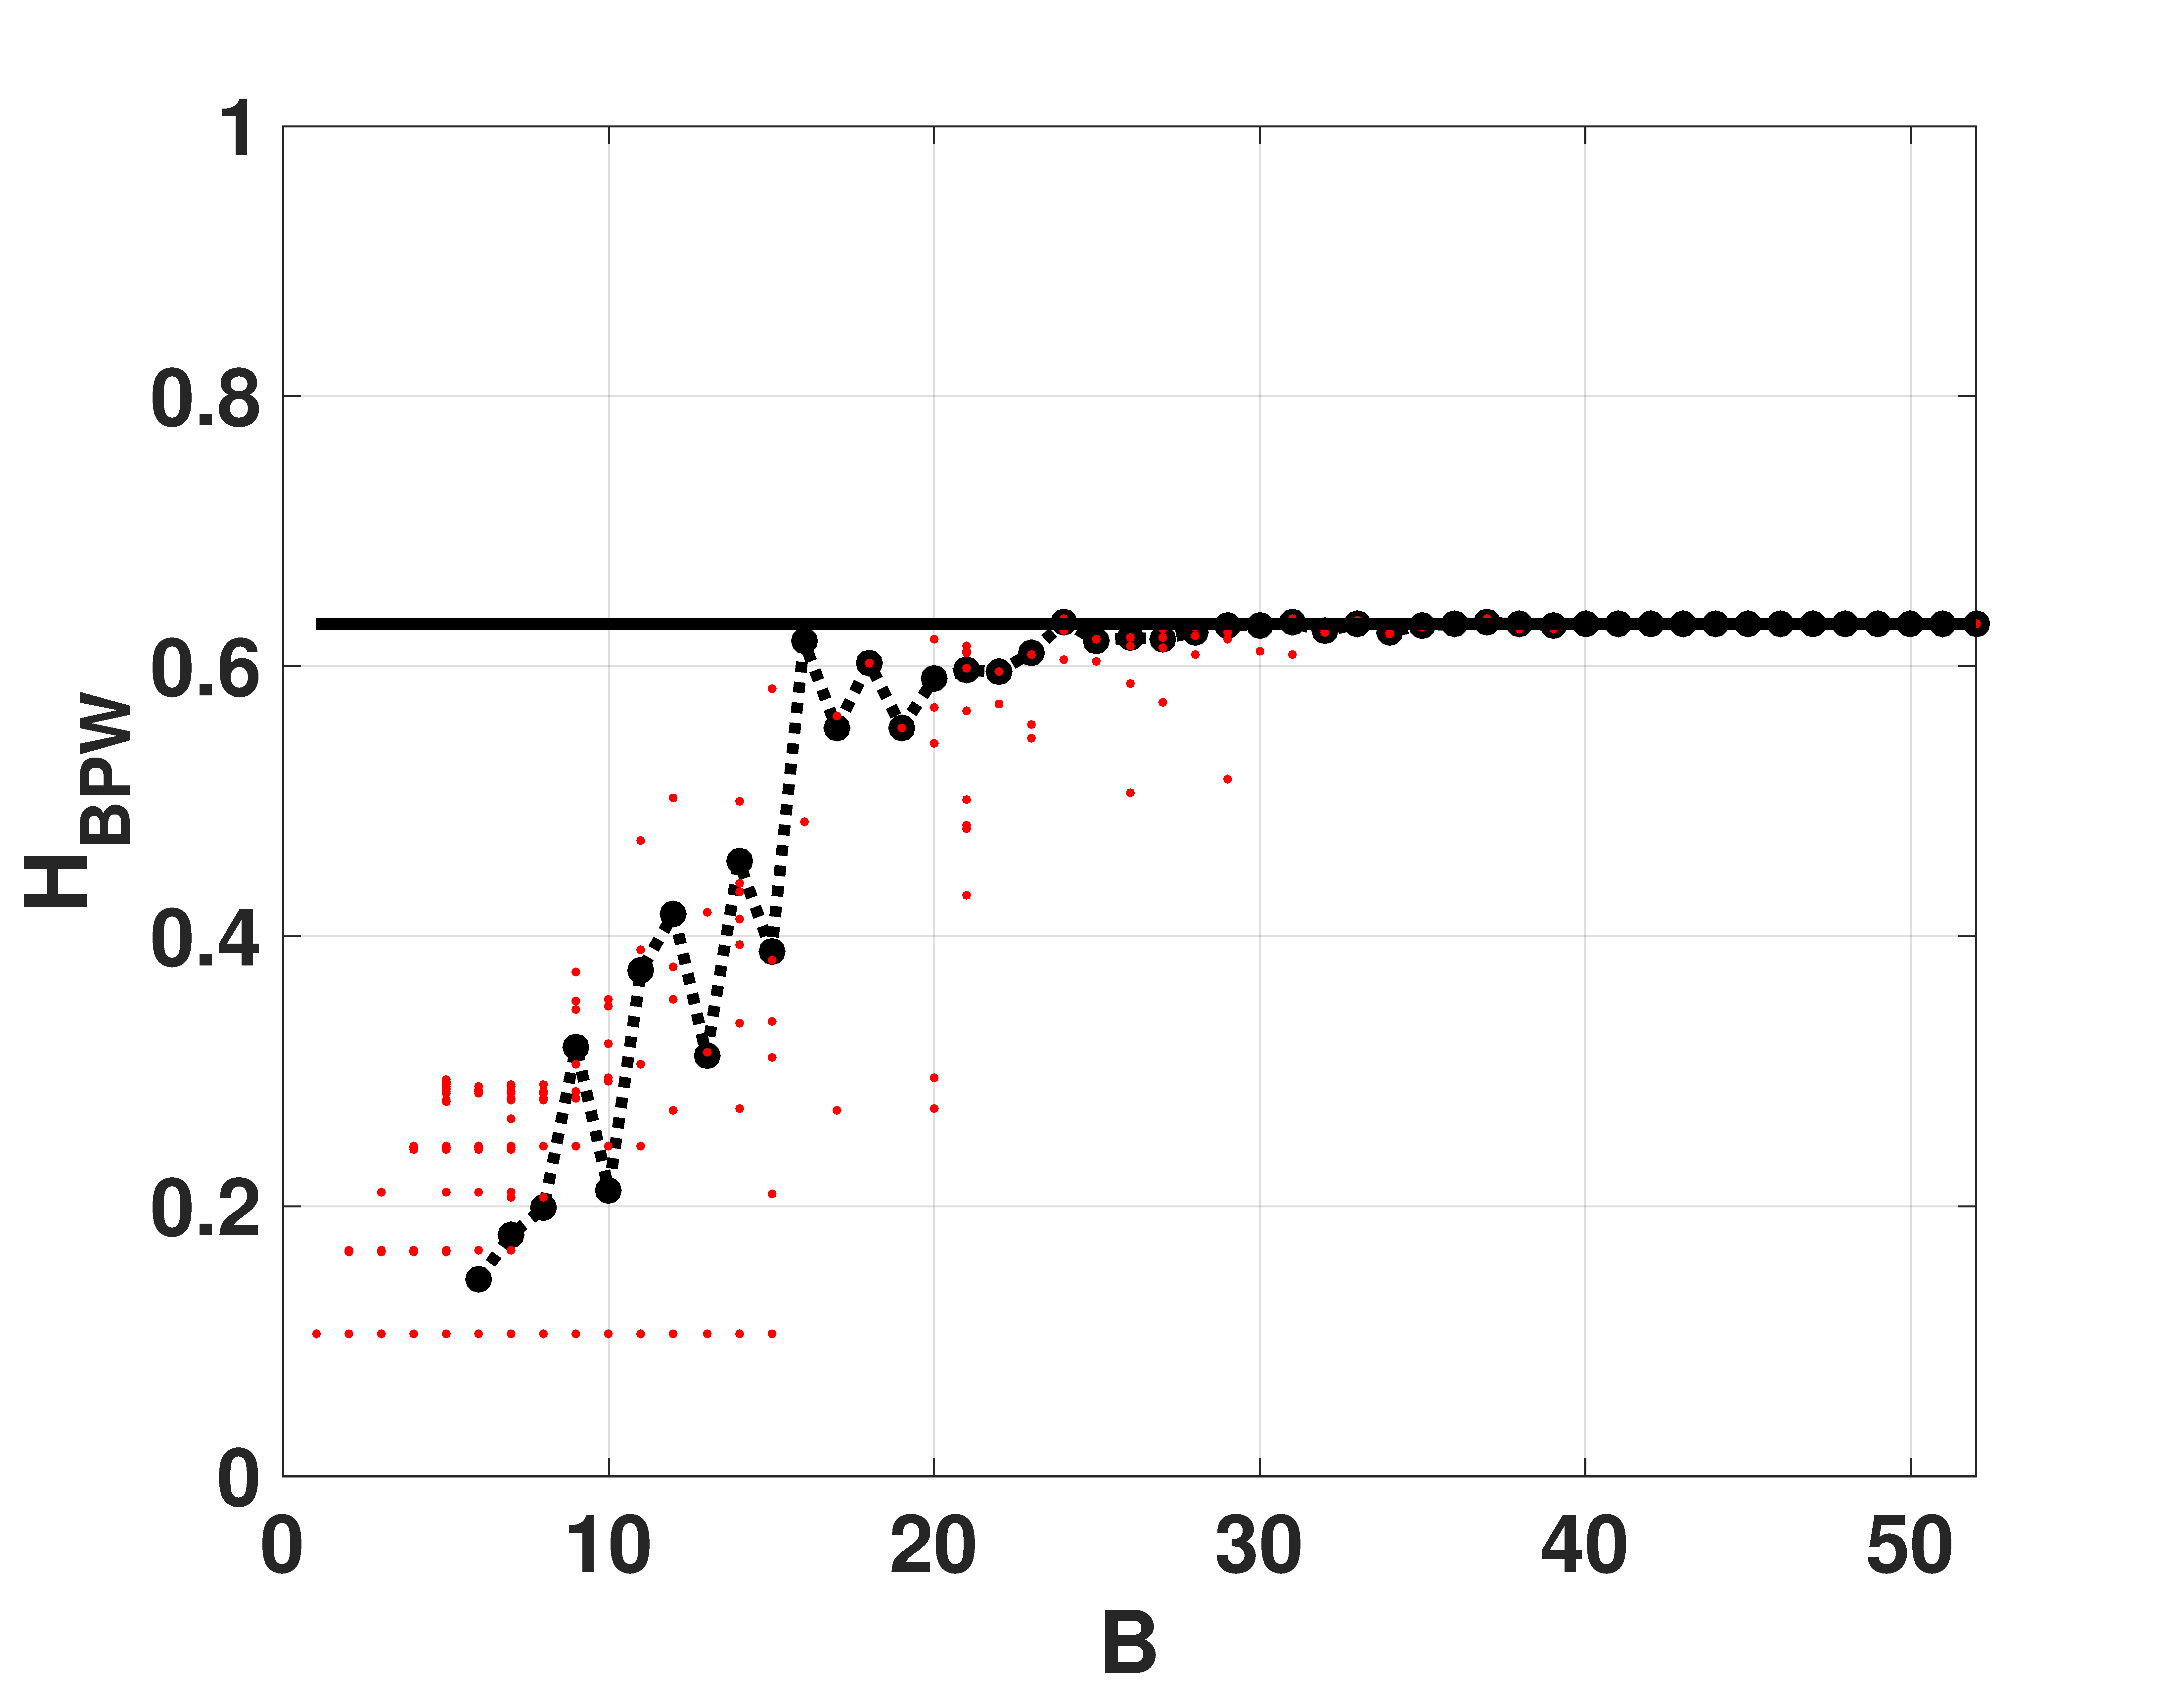
\includegraphics[width=.49\textwidth]{Hbpw_Switch}
	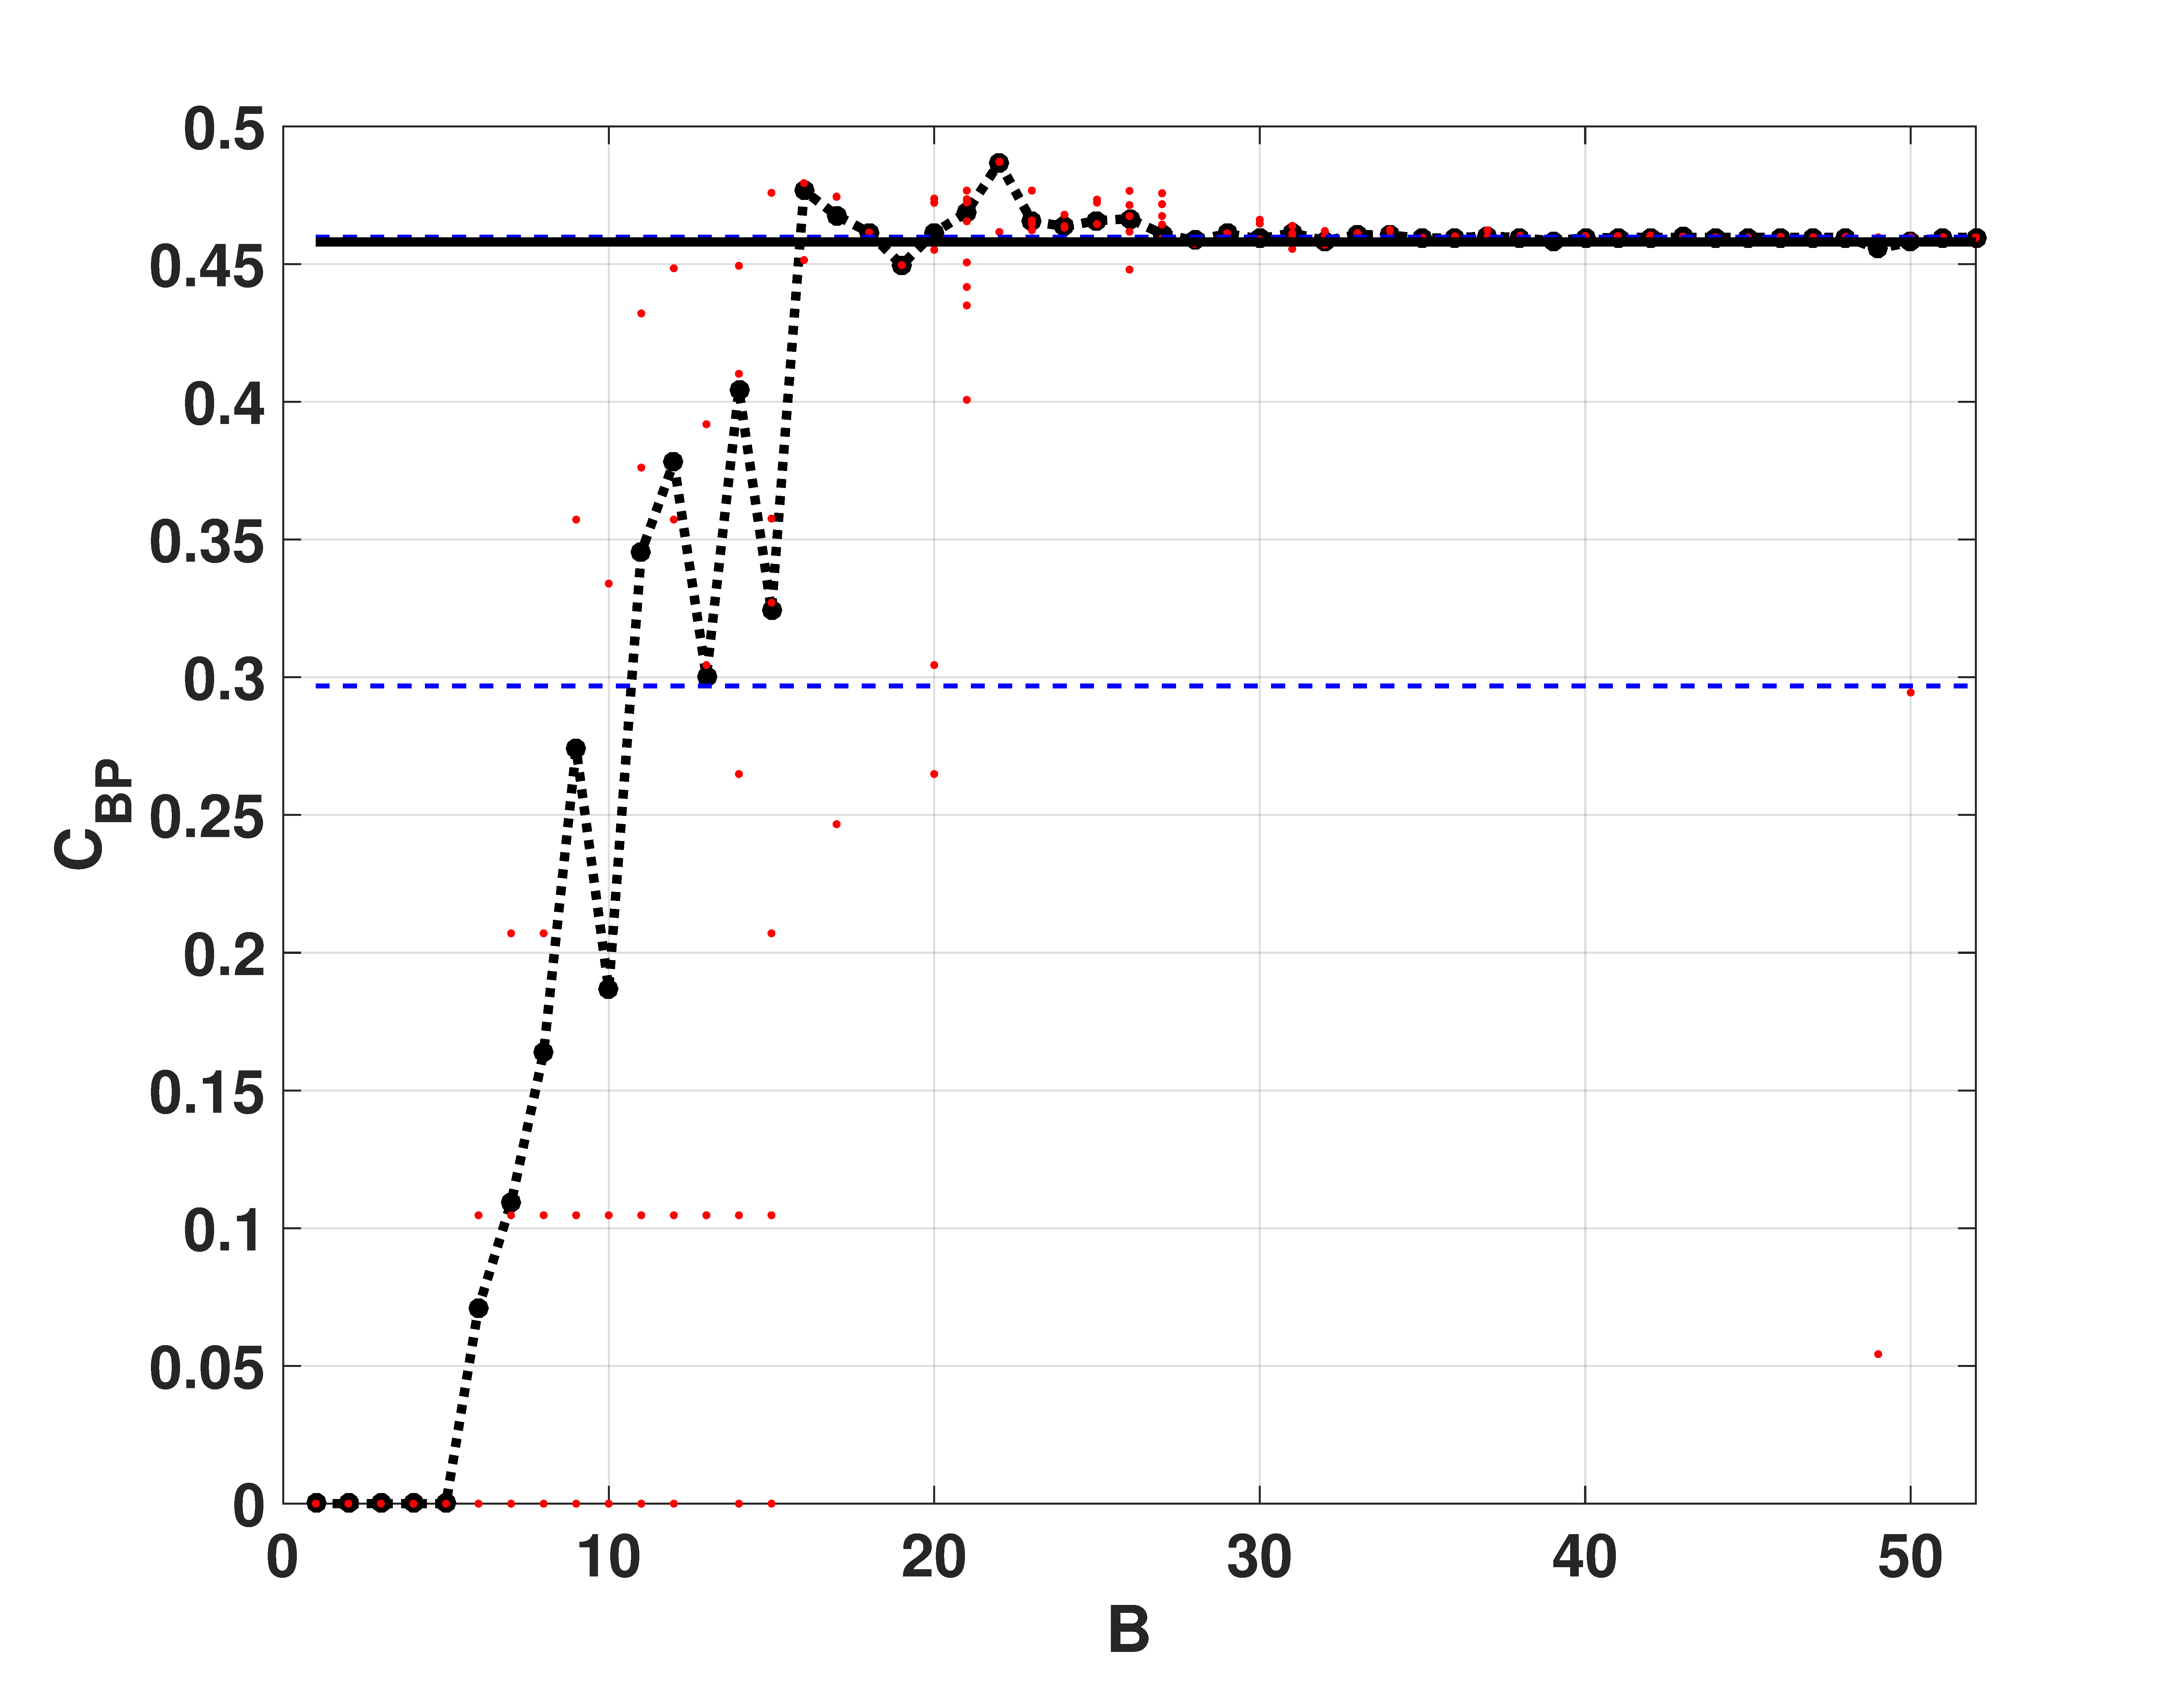
\includegraphics[width=.49\textwidth]{Cbp_Switch}
	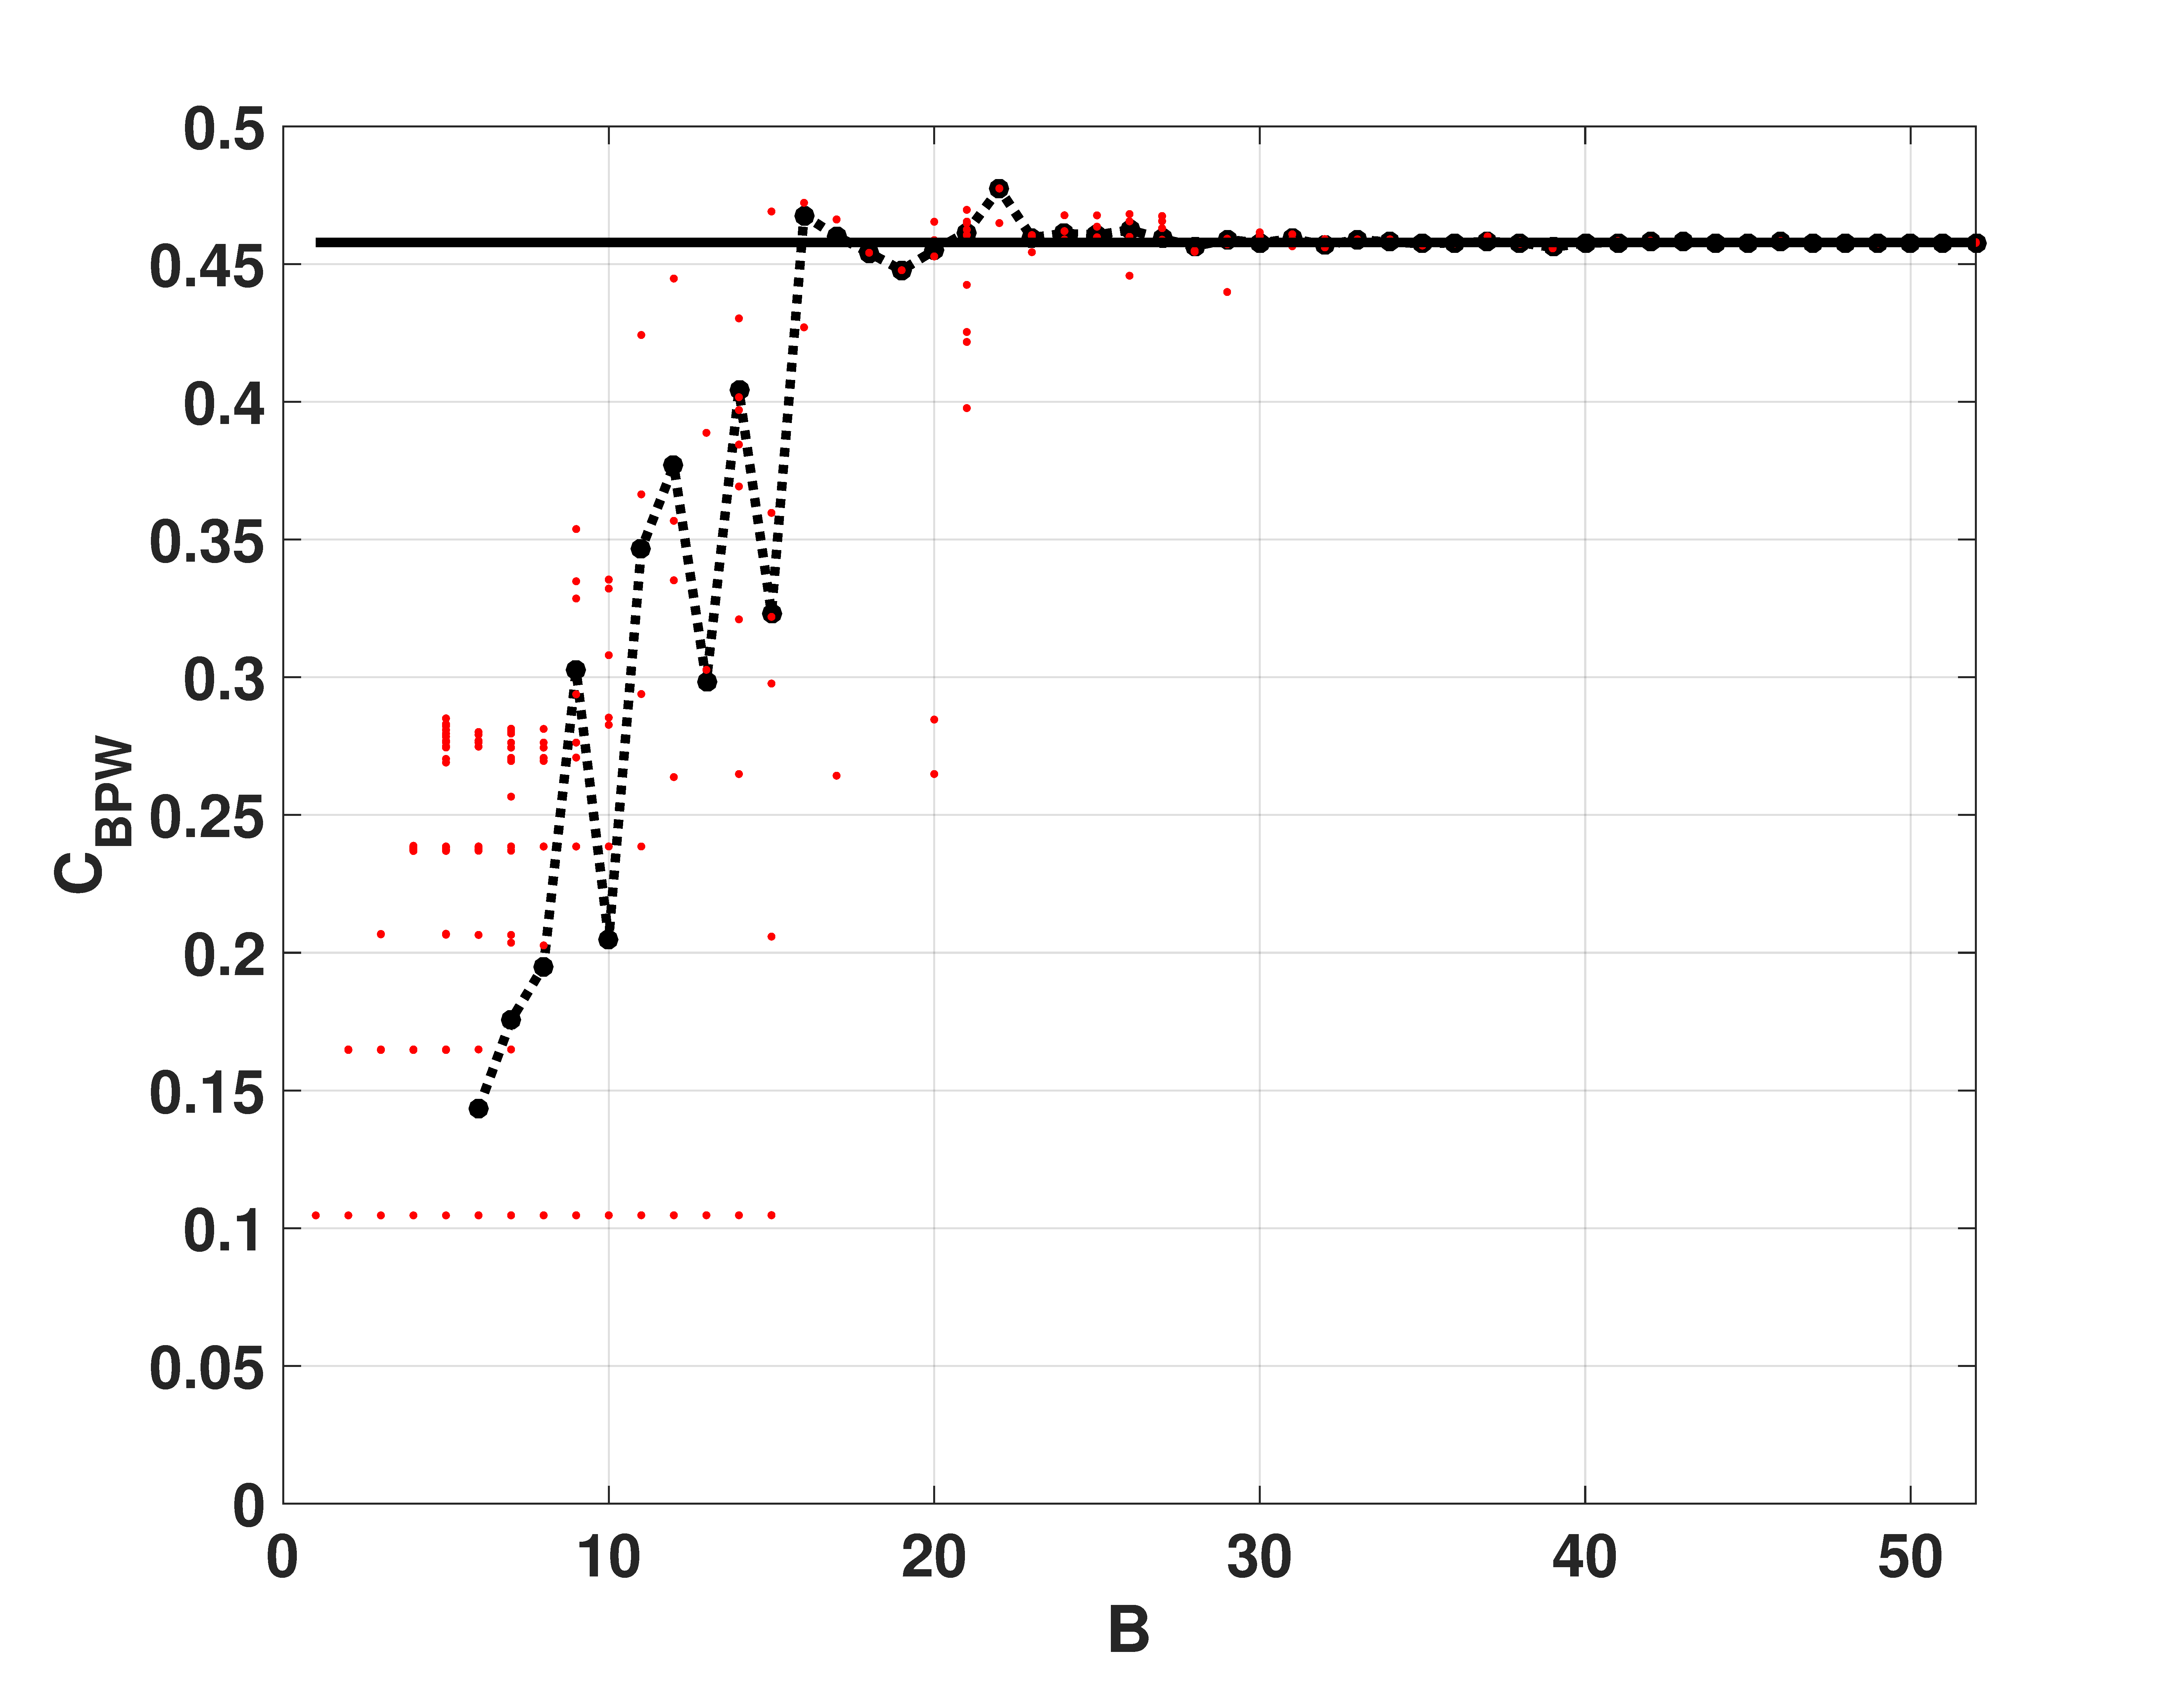
\includegraphics[width=.49\textwidth]{Cbpw_Switch}
	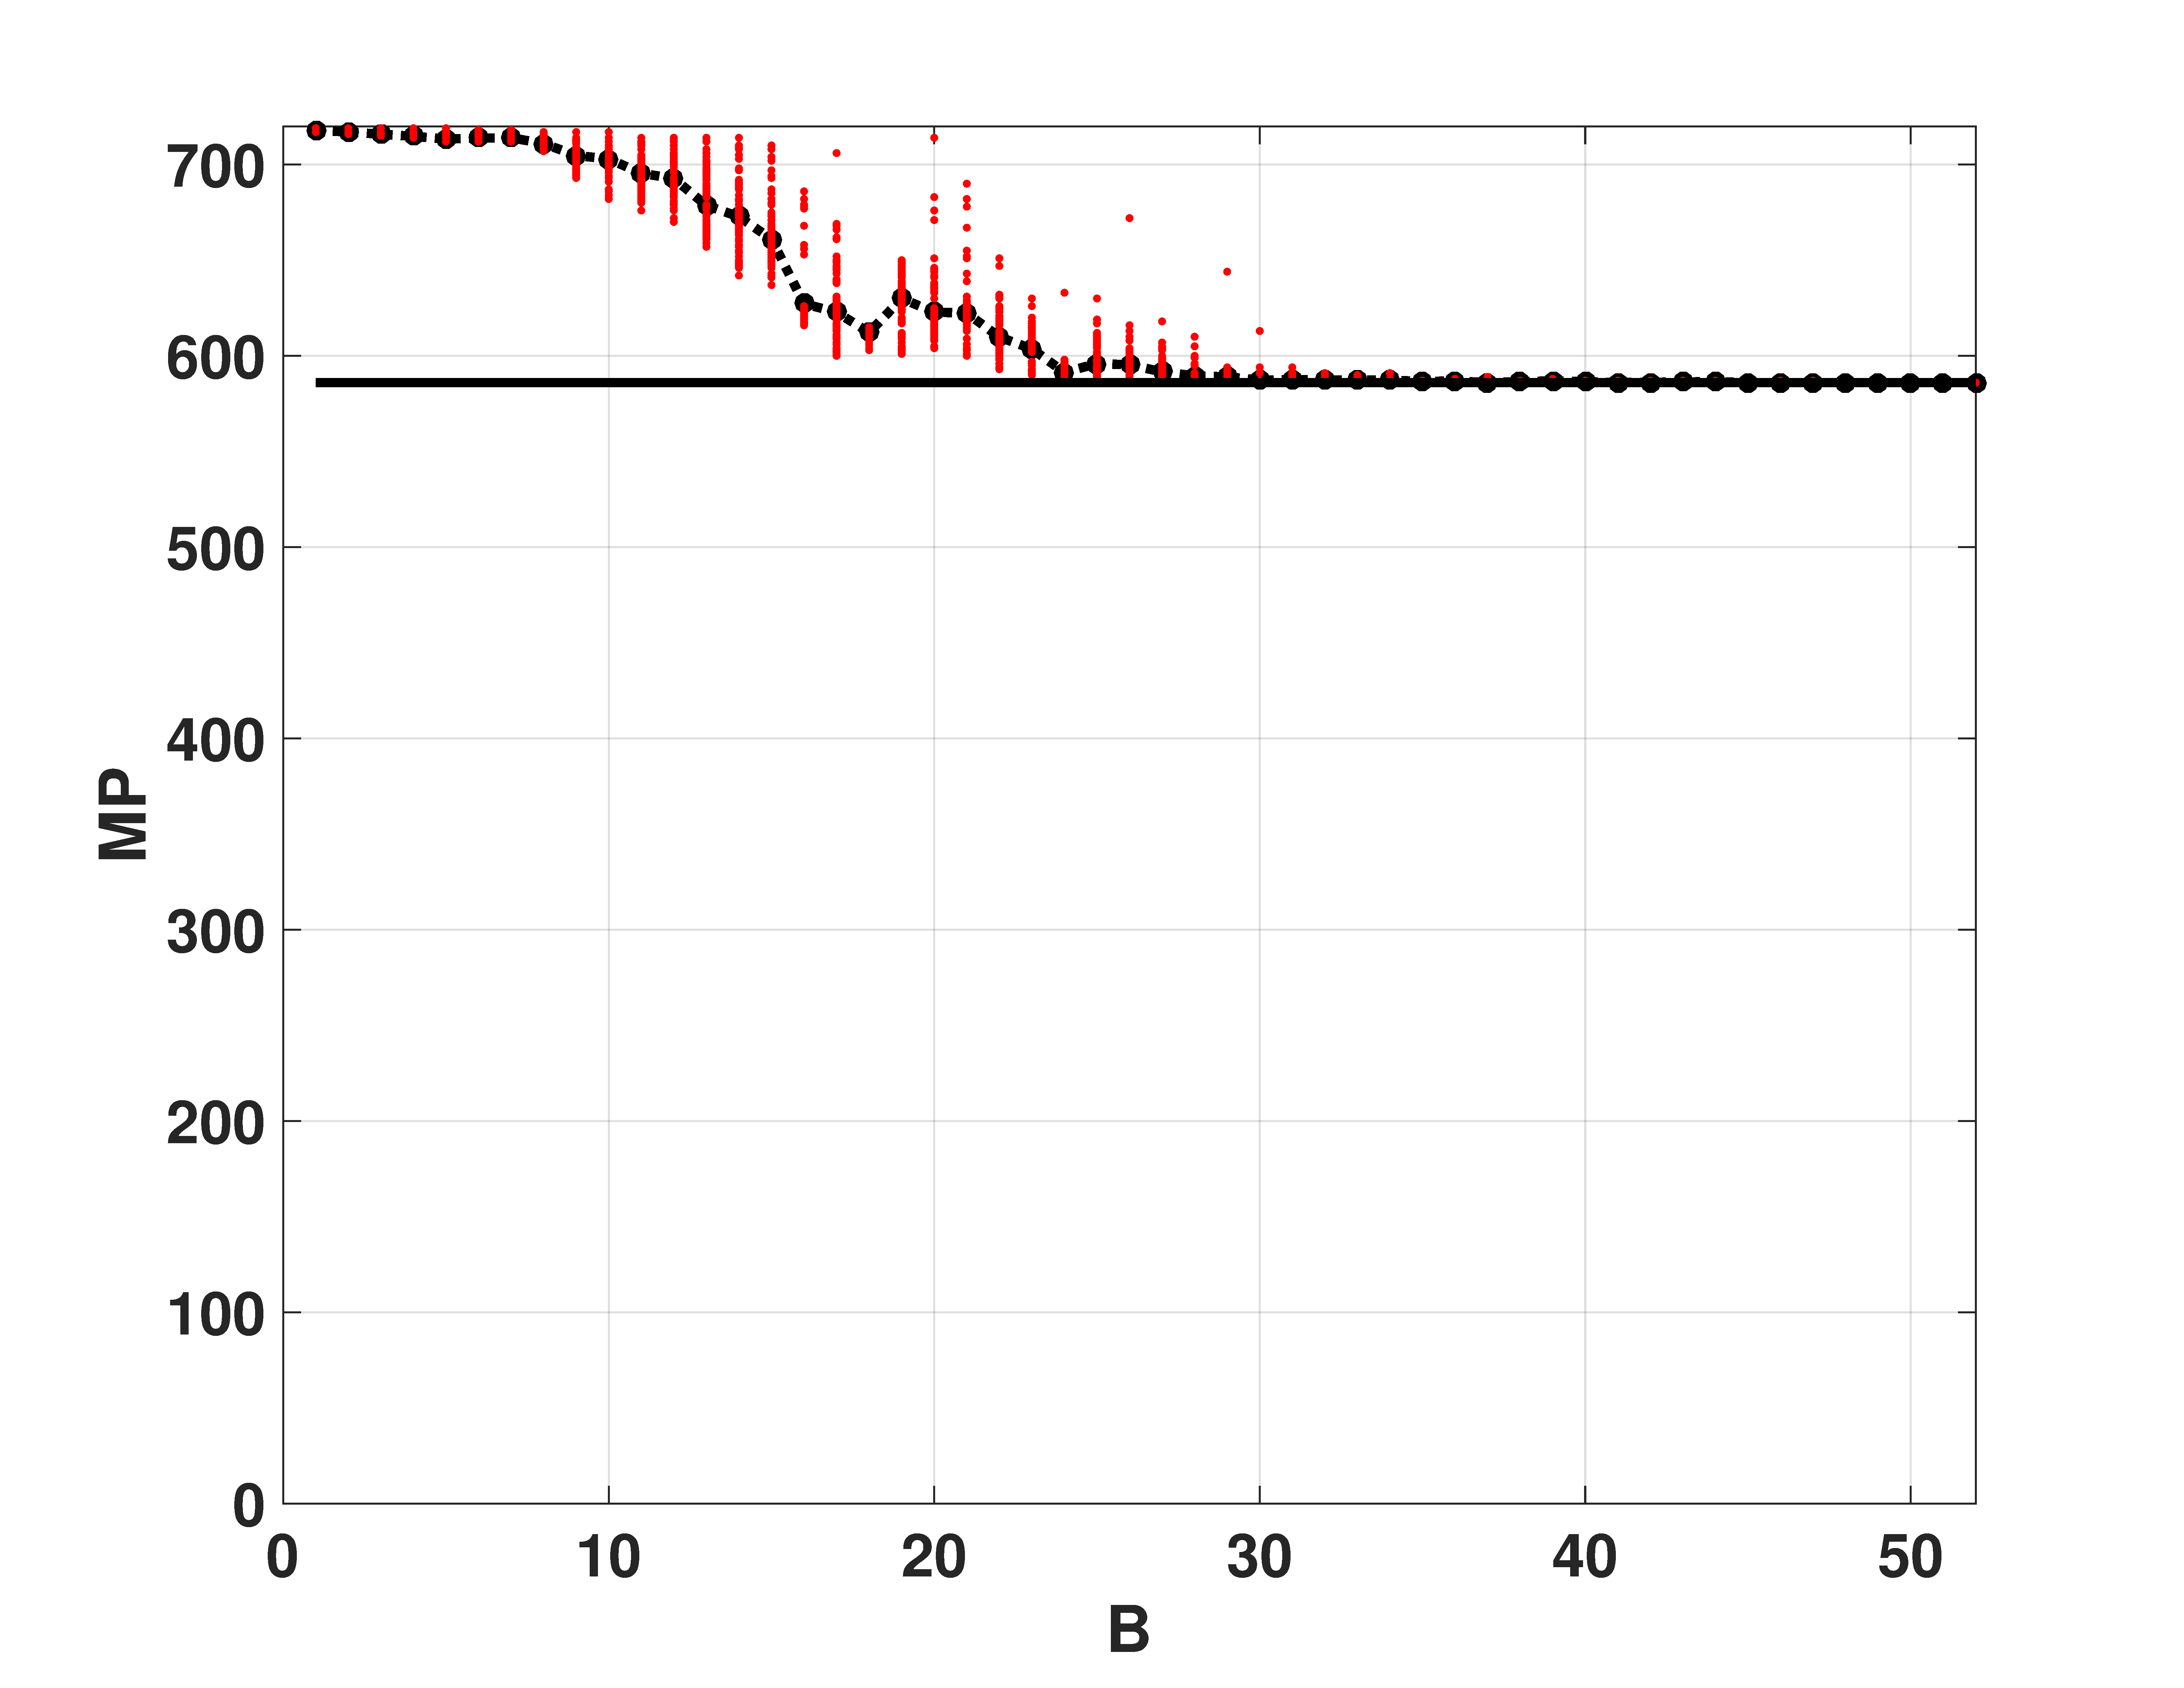
\includegraphics[width=.49\textwidth]{MP_Switch}
	\caption{Statistical properties of the SWITCH map: (a) $H_{val}$ vs $B$ (b) $H_{BP}$ vs $B$ (c) $C_{BP}$ vs $B$ (d) $MP$ vs $B$.}
	\label{fig:SWITCH_QuantiB}
\end{figure}

Double entropy plane $H_{val}$ vs $H_{BP}$ is showed in Fig. \ref{fig:SWITCH_HH}.
The point reached in this plane for SWITCH map is similar to that reached for LOG map.
The mixing is slight better in this case.

\begin{figure}
	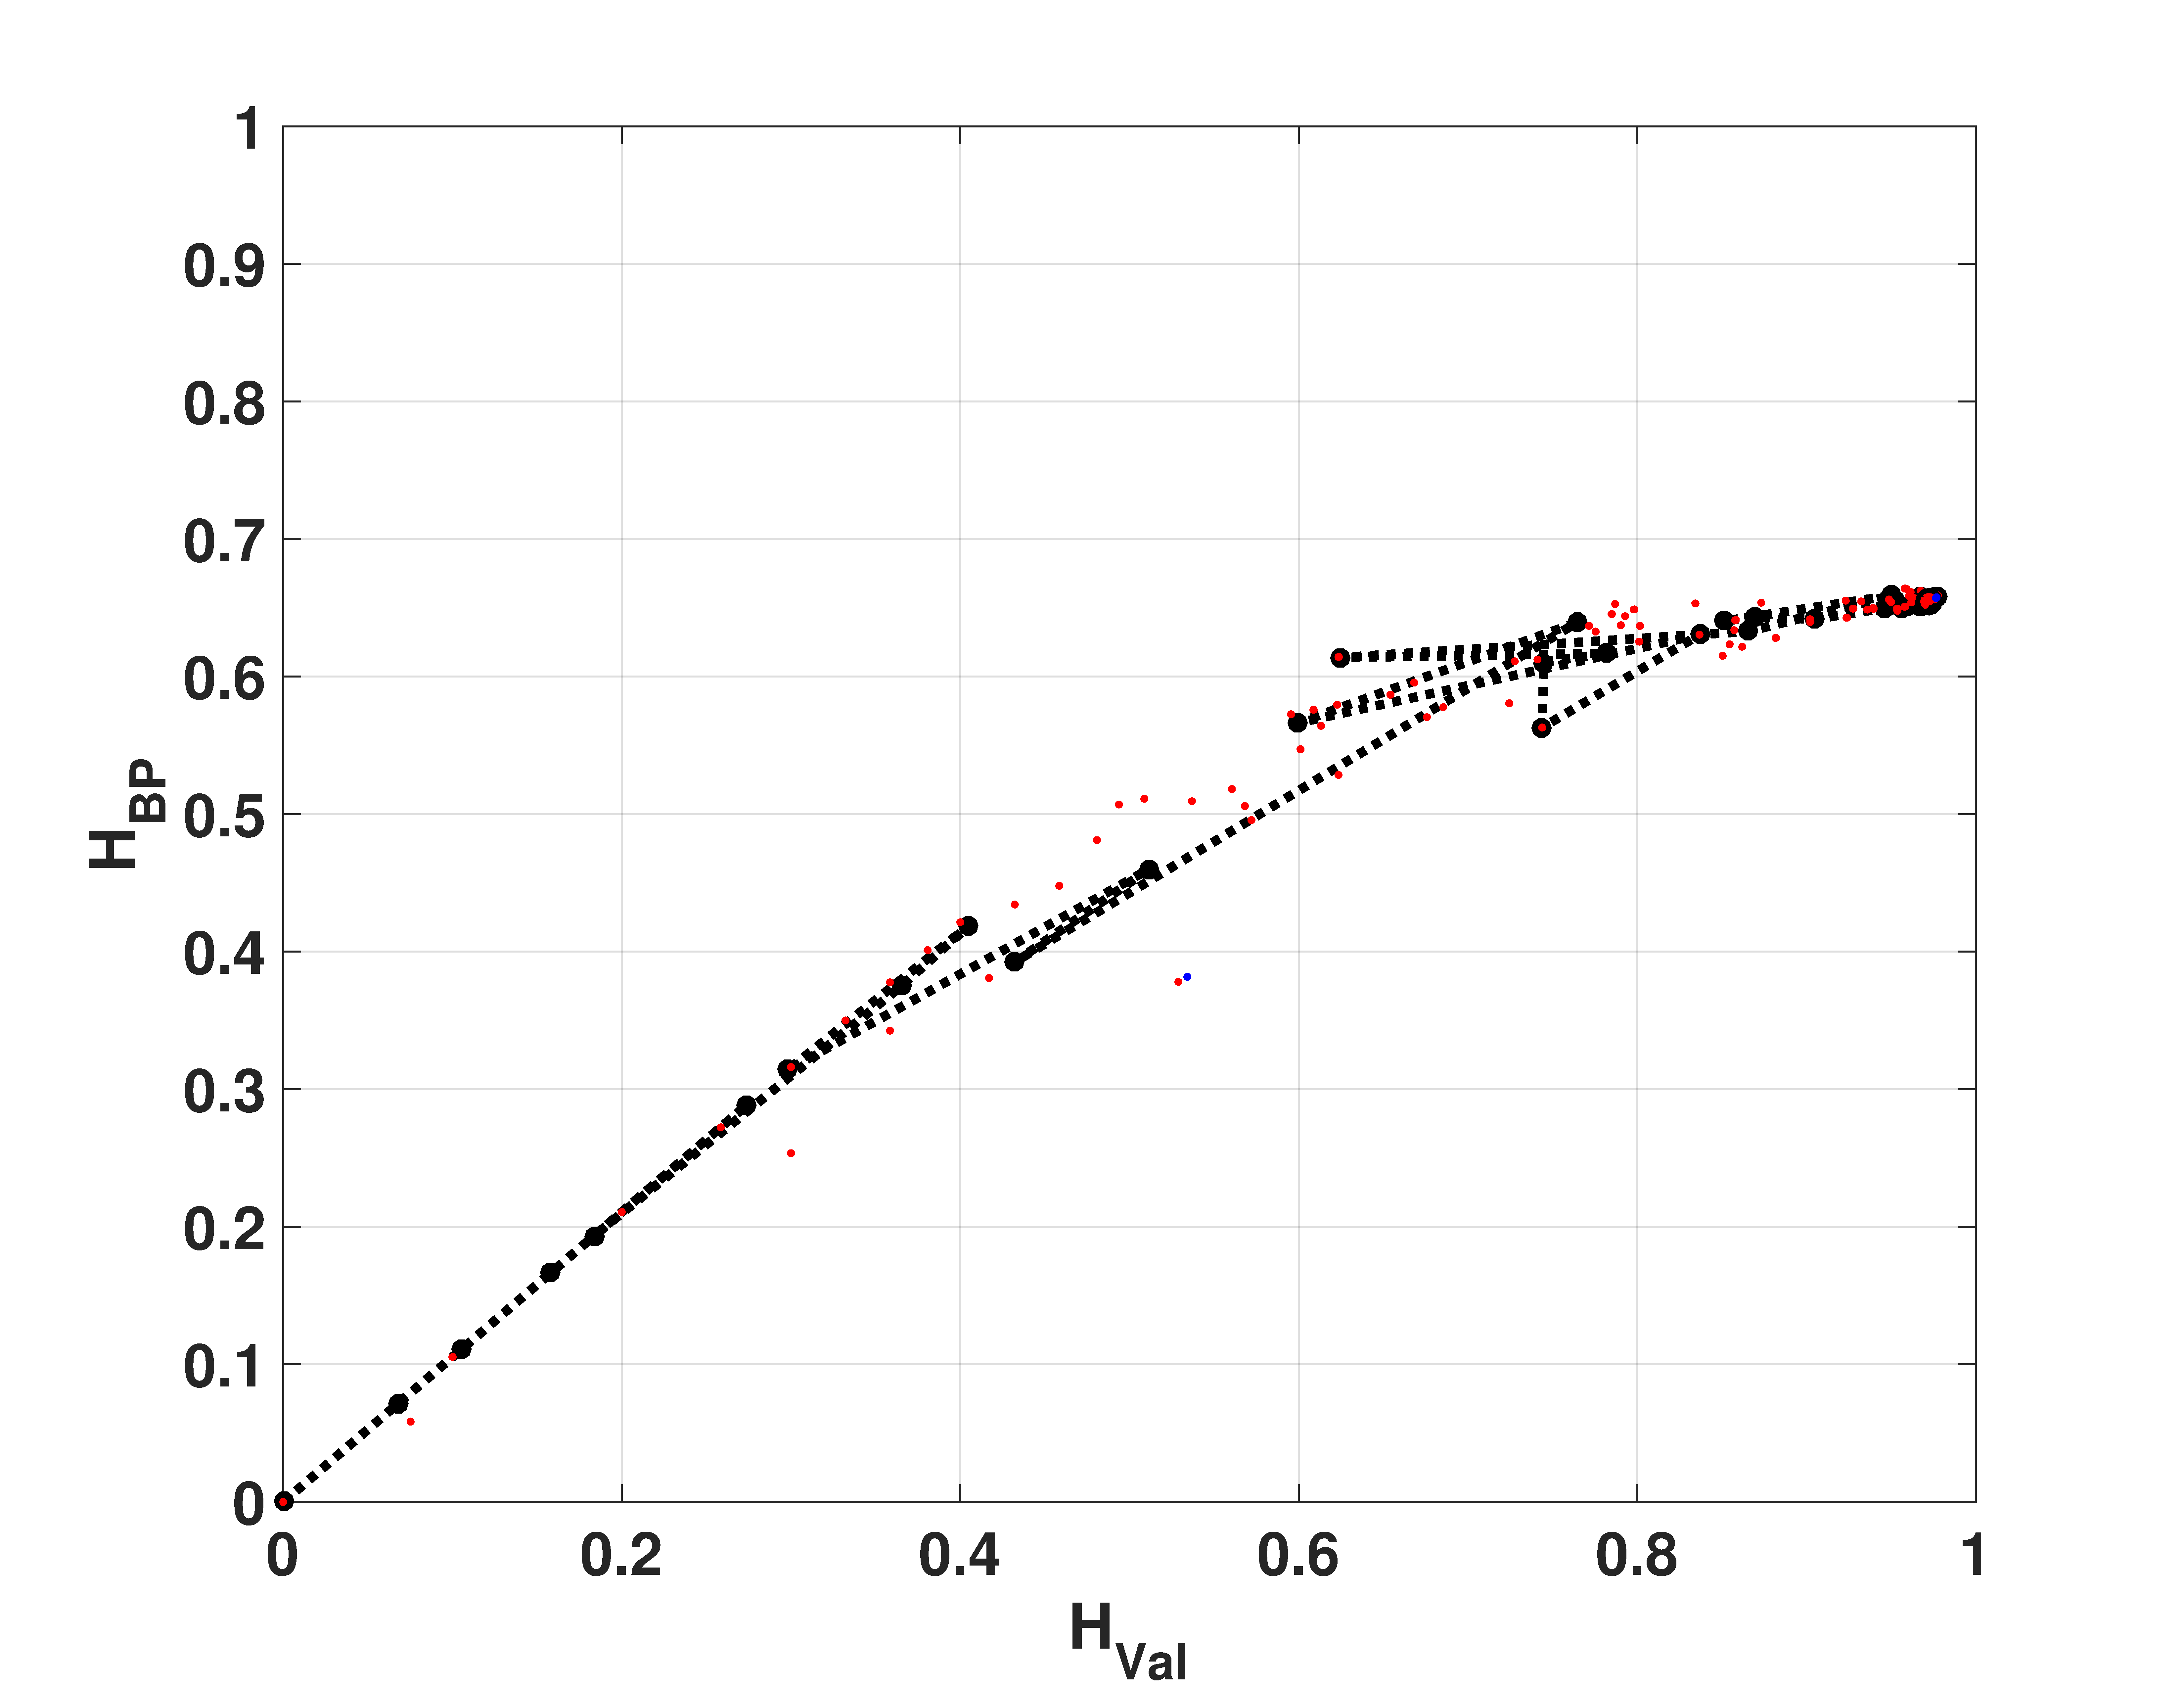
\includegraphics[width=.49\textwidth]{HbpHval_Switch}
	\caption{Evolution of statistical properties in double entropy plane of SWITCH map $H_{val}$ vs $H_{BP}$.}
	\label{fig:SWITCH_HH}
\end{figure}

Entropy-complexity plane $C_{BP}$ vs $H_{BP}$ is showed in Fig. \ref{fig:SWITCH_HC}.
If we compare with the same plane in the case of LOG (Fig. \ref{fig:LOG_HC}. a.), $C_{BP}$ is lower for SWITCH, this fact shows a more random behaviour.

\begin{figure}
	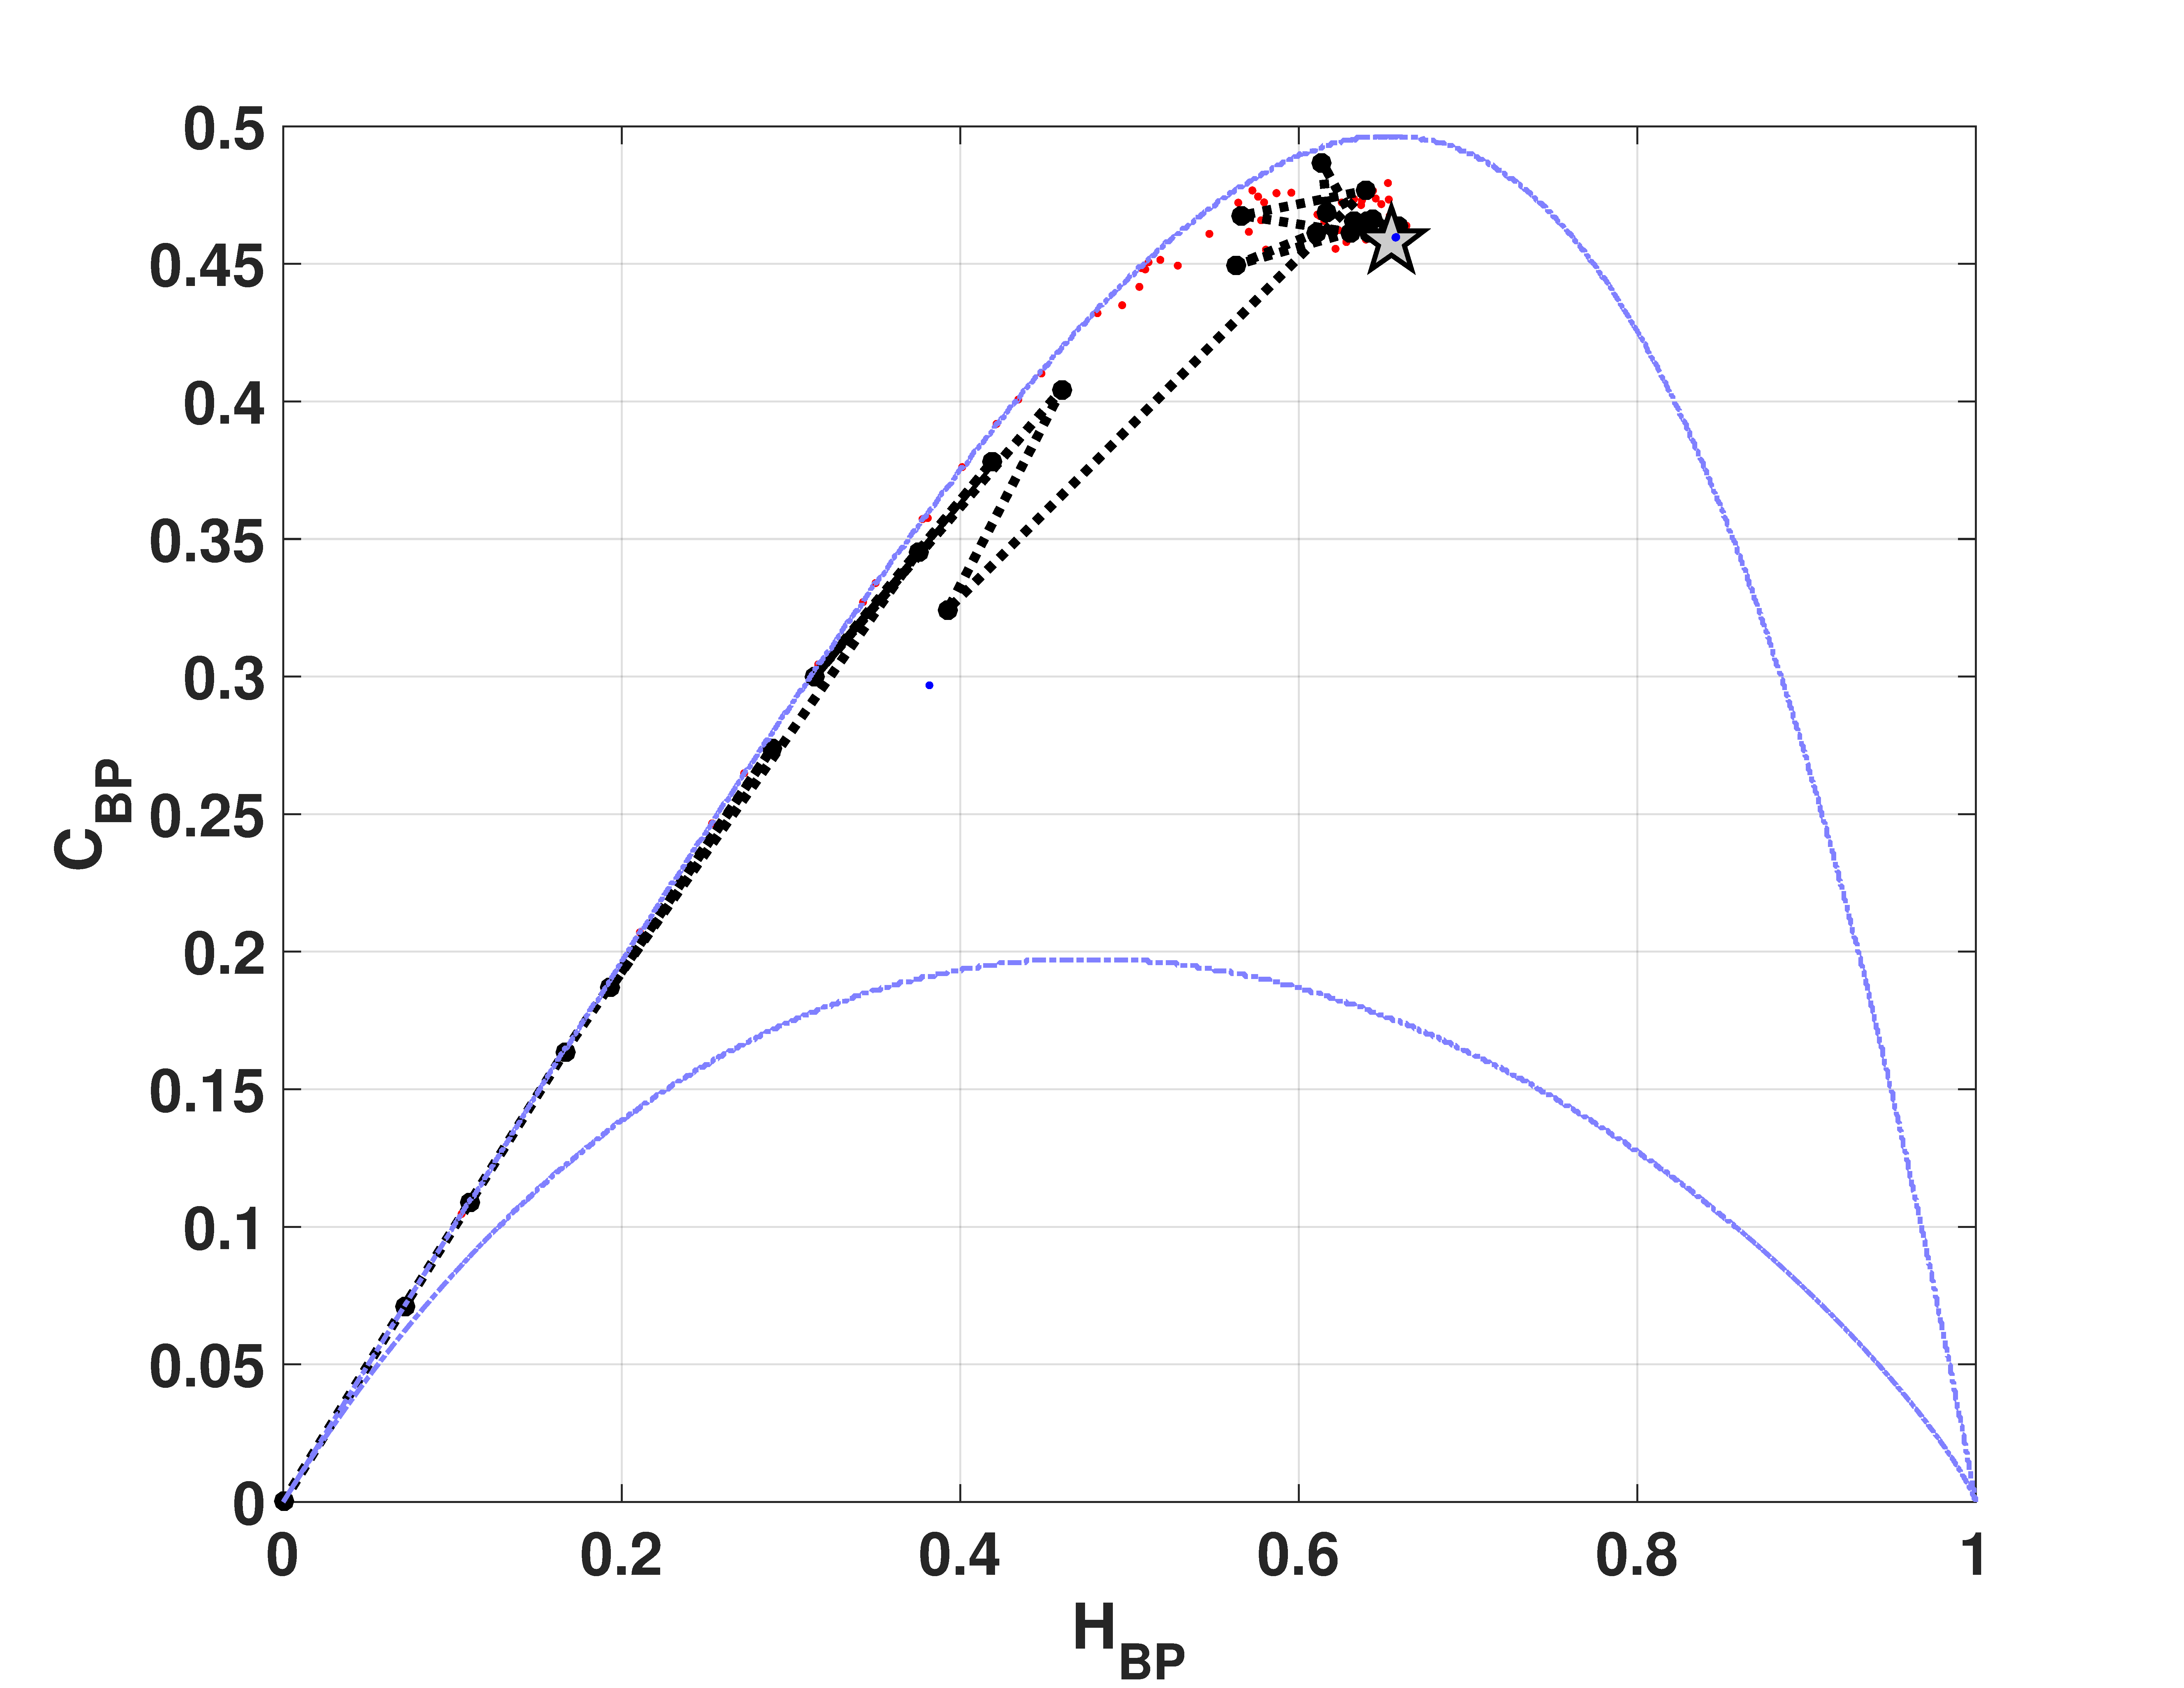
\includegraphics[width=.49\textwidth]{CbpHbp_Switch}
	\caption{Evolution of statistical properties in entropy-complexity plane of SWITCH map $C_{BP}$.}
	\label{fig:SWITCH_HC}
\end{figure}